\documentclass[../../main.tex]{subfiles}
\begin{document}

\subsection*{10.4}
Una spira quadrata di lato $b=9\ cm$, massa $m = 5\ g$ e resistenza $R=10^{-3}\ \Omega$, si muove con velocità costante $v_0 = 5\ \frac{m}{s}$ lungo l'asse z. All'istante t = 0 il suo lato anteriore comincia ad entrare nella regione $x\ge0$ in cui esiste campo magnetico $\vec{B}$, ortogonale al piano della spira, dipendente da x secondo la legge $B(x) = \alpha x$ con $\alpha = 2\ \frac{T}{m}$.\\
Calcolare la forza F(x) che agisce sulla spira, la velocità v(x) della spira e in particolare v(x = b), la carica q che circola nella spira.\\
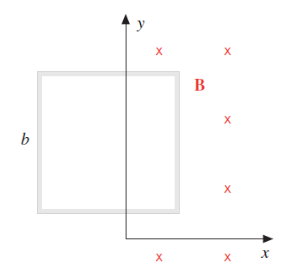
\includegraphics[scale=0.3]{e_10_4.png}
\subsubsection*{Formule utilizzate}
\subsubsection*{Soluzione punto a}
Il campo elettromotore: $\vec{E_i} = \frac{F}{q} = \vec{v}\wedge\vec{B}$\\
Che produce una f.e.m. $\varepsilon_i = \int \vec{E_i} d\vec{s} = vb\alpha x$\\
$i = \frac{\varepsilon_i}{R} = \frac{vb\alpha x}{R}$ in verso antiorario.\\
$F(x) = ibB = b^2\alpha^2x^2\frac{v}{R}$ opposta al moto.\\
$m\frac{dv}{dt} = - \frac{b^2\alpha^2}{R}x^2v$\\
$dv = -\frac{b^2\alpha^2}{mR}x^2 dx$\\
$\int_{v_0}^{v(x)}dv = -\frac{b^2\alpha^2}{mR}\int^x_0x^2dx$\\
$v(x) = v_0 - \frac{b^2\alpha^2}{3mR}x^3=5-2160x^3\ \frac{m}{s}$\\
$v(x = b) = 5-2160 * 0.09^3 = 3.43\ \frac{m}{s}$\\
Usando la legge di Felici:\\
$q = \frac{\Phi_1 - \Phi_2}{R} = \frac{1}{R}b\int_0^b\alpha x dx=\frac{\alpha b^3}{2R} = 0.73\ C$\\
\subsubsection*{Soluzione punto b}
\newpage

\end{document}